
\documentclass{article}
\usepackage{graphicx}
\usepackage{geometry}
\geometry{a4paper, margin=1in}

\begin{document}
\title{Rainfall Forecasting Report}
\author{AI Assistant}
\date{\today}
\maketitle

\section{Introduction}
This report presents the results of rainfall forecasting models.

\section{Results}

\begin{figure}[h!]
    \centering
    \includegraphics[width=0.8\textwidth]{reports/figures/correlation_matrix.png}
    \caption{Correlation Matrix}
    \label{fig:correlation_matrix}
\end{figure}

\begin{figure}[h!]
    \centering
    \includegraphics[width=0.8\textwidth]{reports/figures/knn_pred_vs_actual.png}
    \caption{Knn Pred Vs Actual}
    \label{fig:knn_pred_vs_actual}
\end{figure}

\begin{figure}[h!]
    \centering
    \includegraphics[width=0.8\textwidth]{reports/figures/model_comparison.png}
    \caption{Model Comparison}
    \label{fig:model_comparison}
\end{figure}

\begin{figure}[h!]
    \centering
    \includegraphics[width=0.8\textwidth]{reports/figures/model_performance_comparison.png}
    \caption{Model Performance Comparison}
    \label{fig:model_performance_comparison}
\end{figure}

\begin{figure}[h!]
    \centering
    \includegraphics[width=0.8\textwidth]{reports/figures/random_forest_confusion_matrix.png}
    \caption{Random Forest Confusion Matrix}
    \label{fig:random_forest_confusion_matrix}
\end{figure}

\begin{figure}[h!]
    \centering
    \includegraphics[width=0.8\textwidth]{reports/figures/random_forest_feature_importance.png}
    \caption{Random Forest Feature Importance}
    \label{fig:random_forest_feature_importance}
\end{figure}

\begin{figure}[h!]
    \centering
    \includegraphics[width=0.8\textwidth]{reports/figures/random_forest_pred_vs_actual.png}
    \caption{Random Forest Pred Vs Actual}
    \label{fig:random_forest_pred_vs_actual}
\end{figure}

\begin{figure}[h!]
    \centering
    \includegraphics[width=0.8\textwidth]{reports/figures/residual_analysis.png}
    \caption{Residual Analysis}
    \label{fig:residual_analysis}
\end{figure}

\begin{figure}[h!]
    \centering
    \includegraphics[width=0.8\textwidth]{reports/figures/roc_curve_comparison.png}
    \caption{Roc Curve Comparison}
    \label{fig:roc_curve_comparison}
\end{figure}

\begin{figure}[h!]
    \centering
    \includegraphics[width=0.8\textwidth]{reports/figures/scatter_actual_vs_predicted.png}
    \caption{Scatter Actual Vs Predicted}
    \label{fig:scatter_actual_vs_predicted}
\end{figure}

\begin{figure}[h!]
    \centering
    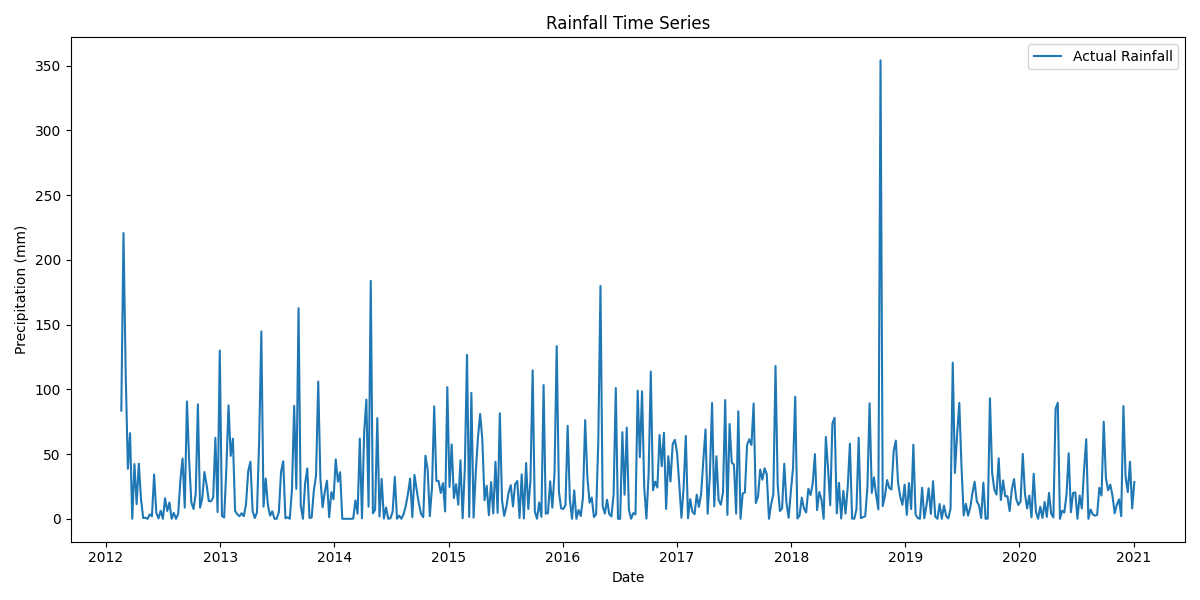
\includegraphics[width=0.8\textwidth]{reports/figures/time_series.png}
    \caption{Time Series}
    \label{fig:time_series}
\end{figure}

\begin{figure}[h!]
    \centering
    \includegraphics[width=0.8\textwidth]{reports/figures/time_series_linear_regression.png}
    \caption{Time Series Linear Regression}
    \label{fig:time_series_linear_regression}
\end{figure}

\begin{figure}[h!]
    \centering
    \includegraphics[width=0.8\textwidth]{reports/figures/xgboost_confusion_matrix.png}
    \caption{Xgboost Confusion Matrix}
    \label{fig:xgboost_confusion_matrix}
\end{figure}

\begin{figure}[h!]
    \centering
    \includegraphics[width=0.8\textwidth]{reports/figures/xgboost_feature_importance.png}
    \caption{Xgboost Feature Importance}
    \label{fig:xgboost_feature_importance}
\end{figure}

\begin{figure}[h!]
    \centering
    \includegraphics[width=0.8\textwidth]{reports/figures/xgboost_pred_vs_actual.png}
    \caption{Xgboost Pred Vs Actual}
    \label{fig:xgboost_pred_vs_actual}
\end{figure}

\section{Conclusion}
These results demonstrate the performance of various rainfall forecasting models.

\end{document}
